\documentclass{article}
\usepackage{iclr2027_conference,times}
\input{math_commands.tex}
\usepackage{hyperref}
\usepackage{url}
\usepackage{booktabs}
\usepackage{graphicx}
\usepackage{amsmath,amssymb}
\usepackage{xcolor}
\newcommand{\todo}[1]{{\color{red}[TODO: #1]}}
\newcommand{\estar}{E^{\star}}

\title{Locating the Missing Evidence: Auditing and Training Spatiotemporal Evidence Acquisition in Video Tool-Use Agents}

\author{Anonymous authors \\ Paper under double-blind review}

\newcommand{\fix}{\marginpar{FIX}}
\newcommand{\new}{\marginpar{NEW}}
\iclrfinalcopy % remove for anonymous submission

\begin{document}
\maketitle

\begin{abstract}
Video tool-use agents can zoom into a frame or replay a time segment, and reinforcement-learned agents such as DeepEyes call these tools frequently while improving accuracy. Whether the returned observations actually enter the decision is a separate question, and recent causal audits have shown that, for image crop-and-zoom, they often do not. Video adds a dimension that images lack: the missing evidence must first be \emph{located} in time. We decompose active video perception into three separately falsifiable layers---\emph{Necessity} (does the coarse observation lack the answer?), \emph{Acquisition} (does the agent's tool call reach the evidence?), and \emph{Utilization} (does the returned evidence change the belief?)---and instantiate each with an intervention rather than a proxy. On VideoNet we machine-certify evidence-gain samples by searching, per question, for the shortest time window whose dense high-resolution frames make a stronger reference model answer correctly; a matched-budget control shows that spending the same visual tokens on uniform frames recovers only half of the gain. Forking real trajectories at the first tool return and substituting a random same-shape return or a blank return, we measure evidence dependence at the step level (probability margin) and at the trajectory level (answer flips), and introduce an \emph{entropy evidence response} that contrasts next-token entropy of the continuation under real versus counterfactual returns, cancelling format uncertainty. \todo{fill fork numbers}. Across 22 certified natural items, the audited agent reaches the evidence window in 5\% of calls and never uses the temporal tool, while the same evidence handed to it raises the correct-answer probability from 0.31 to 0.40 (0.41 to 0.65 for the reference model). We release the certification pipeline, a synthetic twin-pair control set with strictly indistinguishable coarse observations, and a pilot set of evidence-seeking trajectories for supervised fine-tuning. \todo{training result sentence}
\end{abstract}

\section{Introduction}
\label{sec:intro}

Multimodal agents that ``think with images'' interleave reasoning with visual tools: cropping a region, zooming, or---for video---replaying a time segment at higher frame rate. Reinforcement learning with outcome rewards makes such agents call tools more often and answer more accurately~\citep{deepeyes2025,videosearcher2026}. Neither number shows that the tool's \emph{output} participated in the answer. A causal audit of image crop-and-zoom~\citep{illusion2026} recently made this precise: replacing returned crops by random crops, noise, or blank images changes answers far less than accuracy improvements suggest, and most rollouts fall into ``calling without looking'' or ``looking without planning''.

Video changes the shape of the problem in one way that matters. In an image, the evidence is always present in the input at some resolution; the only question is whether the model looks at it. In a video observed through a coarse budget (a handful of uniformly sampled low-resolution frames), the decisive evidence---the take-off edge of a jump, the second contact of bat and ball, the last tuck of a knot---is often \emph{absent} from the observation altogether. An agent must first decide \emph{when} to look before it can decide \emph{where}. This makes the question of whether a sample \emph{needs} additional evidence a property of the sample, not only of the model's calibration, and it makes temporal localization the layer where video agents can fail in a way image agents cannot.

We therefore split active video perception into three layers and give each an intervention (Section~\ref{sec:framework}):
\begin{itemize}
\item \textbf{Necessity.} Is the answer under-determined by the coarse observation, and is there a short time window whose dense, high-resolution frames determine it? We certify this by search rather than annotation (Section~\ref{sec:necessity}) and calibrate the claim against a synthetic control set of \emph{twin} videos whose coarse observations are strictly indistinguishable.
\item \textbf{Acquisition.} Does the agent's own tool call reach that window? We measure temporal hit rates against the certified window set and, more directly, whether the agent's \emph{actual} return helps.
\item \textbf{Utilization.} When the evidence is returned, does the belief move because of its \emph{content}? We fork real trajectories at the first tool return and substitute a random same-shape return or a blank return, keeping the prefix (including the agent's own reasoning and call arguments) fixed.
\end{itemize}

Alongside the probability-margin measure used by prior audits, we introduce an \emph{entropy evidence response} (EER): the difference in mean next-token entropy of the regenerated reasoning under the real versus the counterfactual return. Because both branches share the prefix and the output format, formatting and phrasing uncertainty cancel and what remains is the effect of the evidence on the agent's uncertainty. Unlike a probability margin, EER needs no multiple-choice readout, so it applies to open-ended answers and can serve as a dense, label-free signal for deciding \emph{when} to call.

Our contributions are: (i) a three-layer, intervention-based audit for video tool-use that adds sample-level necessity and temporal acquisition to existing image-level audits; (ii) an automatic certification of evidence-gain samples on VideoNet, with a matched-budget control showing that localization, not more frames, carries the gain; (iii) trajectory-level counterfactual evidence for a representative RL-trained agent, showing \todo{one-line fork result}; (iv) a pilot supervised dataset of evidence-seeking trajectories synthesized from certified windows, and \todo{training result}.

\section{Related Work}
\label{sec:related}

\paragraph{Thinking with images and video tools.} DeepEyes~\citep{deepeyes2025} trains crop-and-zoom with outcome rewards; VideoSearcher~\citep{videosearcher2026} extends multi-tool agentic reasoning to video with a decoupled tool/answer objective; FrameThinker, VideoZoomer and related work add frame selection and temporal tools~\citep{framethinker2025,videozoomer2025}. These works measure success by accuracy and call statistics. AVP~\citep{avp2025} formulates long-video understanding as iterative evidence seeking with a training-free planner--observer--reflector loop on a proprietary model and reports large token savings, but does not test whether the gains depend on the retrieved clips.

\paragraph{Causal audits of tool use.} \citet{illusion2026} audit six thinking-with-images models by substituting tool returns under a fixed prefix and define Visual Evidence Gain as the difference of marginal probability gains under real and counterfactual observations. Their scope is image crop-and-zoom; they explicitly leave frame selection in video and controlled training studies as future work, and they do not define whether a sample requires the tool. FaithEyes~\citep{faitheyes2026} uses an LLM judge to score whether tool results are referenced, without intervention. Our Utilization layer follows the intervention logic of \citet{illusion2026} and extends it to temporal tools; our Necessity layer is the piece these audits lack.

\paragraph{Evidence-grounded training.} Evidence-RL~\citep{evidencerl2026} rewards answers whose support drops when an evidence region is masked relative to matched non-evidence regions; DeFacto~\citep{defacto2025} trains with positive, counterfactual and random-masking variants. Both operate on images where the evidence is present in the input; neither trains a policy to \emph{acquire} evidence that is absent from the initial observation under a budget.

\paragraph{Faithfulness and uncertainty.} Counterfactual tests of chain-of-thought faithfulness~\citep{turpin2023,lanham2023} perturb intermediate reasoning and check whether conclusions change; we apply the same logic to tool returns. Token-level entropy has been used to identify decision points in reasoning~\citep{wang2025entropy} and, in PEA~\citep{pea2026}, to align the positional structure of uncertainty with expert prototypes. We use entropy as a contrastive measurement of whether evidence resolves uncertainty, not as a reward.

\section{Three Layers of Active Video Perception}
\label{sec:framework}

Let $V$ be a video, $q$ a question with answer set $\mathcal{Y}$, and $o_0$ the \emph{coarse observation}: $K$ uniformly sampled frames at a bounded resolution ($K{=}8$, $\le 256\!\cdot\!28^2$ pixels per frame throughout). A tool call $a$ returns an observation $e(a)$: for \texttt{seek}, $n$ dense frames from a time window; for \texttt{zoom}, a crop of one frame at higher resolution. We write $b(y\mid \cdot)$ for the model's belief, read from the next-token distribution over option letters after a forced \texttt{<answer>} prefix, averaged over cyclic permutations of the options to remove position bias.

\paragraph{Necessity (sample property).} A sample is an \emph{evidence-gain sample at budget $K$} for a reference model $M$ if $b_M(y^\star\mid o_0)$ is low and there exists a short window $\estar$ such that $b_M(y^\star\mid o_0, e(\estar))$ is high (Section~\ref{sec:necessity}). We deliberately call this \emph{model-screened} necessity; strict observational indistinguishability---two videos with identical coarse observations and different answers---is established only on a controlled twin-pair set (Section~\ref{sec:twins}).

\paragraph{Acquisition (policy).} Given $\estar$ (or the set of all certified windows), an agent's call $a$ \emph{acquires} evidence if its window intersects a certified window. We report the hit rate and, more directly, the belief gain produced by the agent's own return.

\paragraph{Utilization (policy).} At the first tool return of a real trajectory we fix everything generated so far (system prompt, frames, the agent's reasoning and its call arguments) and substitute the return: real $e$, a random same-shape return $e_{\mathrm{rnd}}$, or a blank return $e_{\mathrm{gray}}$. We measure (a) the step-level margin $g = b(y^\star) - \max_{y\neq y^\star} b(y)$ read immediately after the return, and following \citet{illusion2026} the gain $\mathrm{VEG} = g_{\mathrm{real}} - g_{\mathrm{rnd}}$; (b) whether the regenerated continuation changes its final answer; and (c) the \emph{entropy evidence response}
\begin{equation}
\mathrm{EER} = \bar H_{\mathrm{think}}(e_{\mathrm{rnd}}) - \bar H_{\mathrm{think}}(e),
\end{equation}
where $\bar H_{\mathrm{think}}$ is the mean next-token entropy over the regenerated reasoning tokens, excluding tokens inside tool-call and answer tags. A positive EER means the real evidence resolved more uncertainty than a content-free return of the same shape; because both branches share the prefix and format, EER isolates the evidence's effect on uncertainty without a multiple-choice readout.

\section{Certifying Evidence-Gain Samples}
\label{sec:necessity}

\paragraph{Screen.} For each question we compute the belief curve $b(y^\star\mid o_0^{(k)})$ for $k\in\{2,4,8,16,32\}$ frames and for $k{=}8$ at higher resolution, plus a text-only belief. Questions solved from text alone or already solved at $k{=}8$ ($b\ge 0.7$, correct) are set aside; the latter form the $N{=}0$ control group.

\paragraph{Window search.} For the remaining candidates we slide windows of width $10/20/30\%$ of the duration (24 positions), append $n{=}6$ dense high-resolution frames from each window to $o_0$, and take the shortest window with $b(y^\star)\ge 0.6$, correct, and a gain of at least $0.25$ over $o_0$ as $\estar$. We keep the full set of windows meeting the criterion for hit-rate computation, and we re-measure $b(y^\star\mid o_0,e(\estar))$ with independent option permutations in the audit stage, since the search value is subject to winner's curse (0.77 at search time versus 0.65 on re-measurement).

\paragraph{Matched-budget control.} Because $e(\estar)$ adds visual tokens, we compare against \emph{dense\_matched}: the same token budget spent on additional uniformly sampled coarse frames ($k{=}26$).

\paragraph{Result on VideoNet.} On 339 questions with local video (37 domains, median 5.9\,s), the reference model Qwen3.5-9B certifies 22 evidence-gain samples (18 of which are solved by no uniform budget up to 32 frames and no resolution increase), 85 already-solvable controls, 32 borderline, and 196 unsolved-even-with-evidence. The median $\estar$ width is 10\% of the duration---about 0.4\,s. Windows found independently by two different models intersect or are adjacent in 62\% of the certified items against a 19\% permutation baseline, and windows found by the reference model transfer to the audited model (Table~\ref{tab:audit}). Using the weaker audited model as its own certifier yields only 8 samples and labels 15 of the 22 as unsolvable, which is why certification and audit use different models.

\begin{figure}[t]
\centering
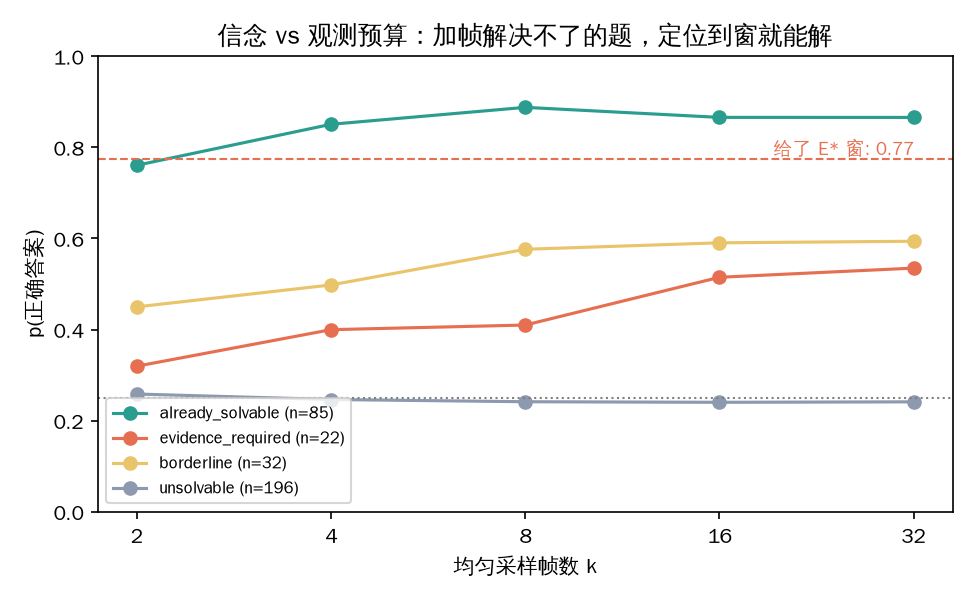
\includegraphics[width=0.62\linewidth]{../natural/out/figs/fig1_budget_curve_qwen35.png}
\caption{Belief in the correct answer versus uniform frame budget for the four screening groups (reference model). Evidence-gain samples saturate at $0.54$ with 32 uniform frames but reach $0.65$ (re-measured) with the six dense frames of $\estar$.}
\label{fig:budget}
\end{figure}

\section{Twin Pairs: A Control Set with Strict Indistinguishability}
\label{sec:twins}
\todo{5 synthetic twin pairs (occlusion release, tiny tag $\times$2, rolling direction, flashed symbol); C1--C4 certification; numbers from pilot/eval/results\_final.json. Keep as positive control, not as the main claim.}

\section{Experiments}
\label{sec:exp}

\subsection{Utilization: evidence handed to the agent}
\begin{table}[t]
\centering
\small
\begin{tabular}{llccccccc}
\toprule
Model & Set & none & $\estar$ & decoy & gray & dense\_matched & EEG & ERG\\
\midrule
DeepEyes-7B & evidence-gain ($n{=}22$) & 0.31 & \textbf{0.40} & 0.31 & 0.33 & 0.33 & $+0.30$ & $+0.14$\\
DeepEyes-7B & control ($n{=}40$) & 0.63 & 0.67 & 0.64 & 0.63 & 0.64 & $+0.04$ & $-0.05$\\
Qwen3.5-9B & evidence-gain ($n{=}22$) & 0.41 & \textbf{0.65} & 0.34 & 0.44 & 0.52 & $+0.70$ & $+0.68$\\
Qwen3.5-9B & control ($n{=}40$) & 0.90 & 0.89 & 0.88 & 0.88 & 0.89 & $+0.02$ & $0.00$\\
\bottomrule
\end{tabular}
\caption{Mean belief in the correct answer when the coarse observation is followed by different returns (single-turn readout). Values are probabilities, not accuracies. \textbf{Caveat}: decoy here is the worst same-width window by the certifier's belief, which biases EEG upward; Section~\ref{sec:fork} replaces it by a random return. \todo{re-run with random decoy and the same protocol for controls}}
\label{tab:audit}
\end{table}

\subsection{Acquisition: the agent's own calls}
On the 22 certified items, the audited agent (zoom and seek available, Chinese prompts, up to four turns) reaches a certified window in 1 of 22 calls (4 of 22 when all certified windows are counted), uses the temporal tool in 1 of 22 trajectories, makes exactly one zoom per question, and states its conclusion before the call in 12 of 22 trajectories. Its zoom frames sit at the median 42\% of the video regardless of where $\estar$ is (median 40\%); with 10\%-wide windows this coincides only by chance.

\subsection{Trajectory forks at the first tool return}
\label{sec:fork}
\todo{Table: real / random / gray branches --- accuracy, step-level margin, VEG, $\bar H_{\mathrm{think}}$, EER, answer-flip rate; separately for evidence-gain and control items. Report the fraction of trajectories that are evidence-dependent (VEG$>0.1$ or flip) and corr(VEG, EER). Numbers from natural/out/fork.jsonl.}

\subsection{Entropy dynamics}
Across 62 trajectories the first \texttt{<tool\_call>} appears at a median 39\% of the output (IQR 32--40\%), 62\% of the top-20\% high-entropy tokens precede it, and the top-20\% positional histogram is indistinguishable between correct and incorrect answers and between evidence-gain and control items. We report these as descriptive statistics; the causal statements rest on Section~\ref{sec:fork}. \todo{replace ent\_post computed from the tool-call token with the continuation-only value from fork.jsonl}

\subsection{Baselines for localization}
\todo{uniform $k$, random window, motion-energy window, model-reported window + programmatic crop, native video agent; cost in visual tokens, text tokens, latency; Pareto plot.}

\section{Learning to Acquire Evidence}
\label{sec:method}
\paragraph{Supervised trajectories from certified windows.} For each certified item we synthesize a two-turn trajectory: a first reasoning step that states what the coarse frames show and which detail or moment is missing, a \texttt{seek} call on $\estar$, and a second reasoning step that reads the returned frames and answers. Reasoning text is written by the reference model conditioned only on the frames it is allowed to see; samples whose first step leaks the answer are discarded. \todo{size of sft\_pilot\_clean.jsonl; SFT result}
\paragraph{Counterfactual-branch RL.} \todo{per-branch correctness reward (real branch: $y^\star$; twin branch obtained by the policy's own call in the twin environment); budget cost on $N{=}0$ items; no reward on answer change or entropy.}

\section{Limitations}
Certification is model-relative; strict indistinguishability holds only for the twin-pair control set. The natural set is small (22 items; \todo{expand}) and drawn from short trimmed clips where evidence gaps are rare by construction. The audited agent is an image tool model extended with a video interface, so part of its failure may reflect transfer rather than an inherent limit; native video agents should be added. Entropy statistics describe behaviour and are used only contrastively.

\bibliography{references}
\bibliographystyle{iclr2027_conference}

\appendix
\section{Certification protocol details}
\todo{thresholds, permutations, window grid, winner's-curse re-measurement}
\section{The 22 certified items}
\todo{table from natural/out/table\_required22.json}
\end{document}
